\documentclass[12pt,a4paper]{article}
\usepackage{appendix}
\usepackage[utf8]{inputenc}
\usepackage[french]{babel}
\usepackage[T1]{fontenc}
\usepackage{amsmath}
\usepackage{amsfonts}
\usepackage{amssymb}
\usepackage{graphicx}
\usepackage[left=2cm,right=2cm,top=2cm,bottom=2cm]{geometry}
\usepackage{ccaption}
\author{Malenfer François, Carbonneau Danaël}

\usepackage[Glenn]{fncychap}

\usepackage{fancybox}

\usepackage{multicol}
\usepackage[hidelinks]{hyperref}

\usepackage[dvipsnames]{xcolor}
\usepackage{tcolorbox}
\usepackage{listings}
\usepackage{algorithm,algorithmic}



	
	
\definecolor{darkWhite}{rgb}{0.94,0.94,0.94}
 
\lstset{
  aboveskip=3mm,
  belowskip=-2mm,
  backgroundcolor=\color{darkWhite},
  basicstyle=\footnotesize,
  breakatwhitespace=false,
  breaklines=true,
  captionpos=b,
  commentstyle=\itshape \color{teal},
  extendedchars=true,
  framexleftmargin=16pt,
  framextopmargin=3pt,
  framexbottommargin=6pt,
  frame=tb,
  keepspaces=true,
  keywordstyle=\bfseries \color{orange},
  otherkeywords={module,open,Int32},
  language=caml,
  morekeywords={*,...},
  numbers=left,
  numbersep=10pt,
  numberstyle=\tiny\color{teal},
  rulecolor=\color{black},
  showspaces=false,
  showstringspaces=false,
  showtabs=false,
  stepnumber=1,
  stringstyle=\color{gray},
  tabsize=4,
  title=\lstname,
}	
	
	
	
	
\usepackage{enumitem}
\usepackage{pifont}
\setitemize[1]{font=\bfseries, label= \color{teal} \ding{227}  }
\setitemize[0]{font=\bfseries, label= \color{olive} \ding{216}  }


\begin{document}


\begin{titlepage}
\newcommand{\HRule}{\rule{\linewidth}{0.5mm}}



\center 
\bigskip
\textsc{\LARGE\textbf{
\color{teal}Sorbonne Université}
}
 \\[4cm]
 {\color{Bittersweet}\HRule} \\[0.4cm]
{ \huge \bfseries \color{darkgray} Devoir de Programmation \\[0.15cm] }
\textbf{Algorithmique Avancée}
{\color{Bittersweet}\HRule} \\[0.5cm]

{\color{darkgray} François Malenfer (28706664), Danaël Carbonneau (28709878)} \\[3cm]

\begin{huge}
{\fontfamily{lmtt}\selectfont
Implémentation de structures de données de recherche (en OCaml)
}
\end{huge}


\vfill

\textit{Enseignant : Antoine Genitrini}

Master Informatique, Semestre 1, septembre - janvier 2023 - 2024 \\ [1cm]

\end{titlepage}



\tableofcontents

\newpage

\section{Échauffement}
Le code correspondant à cette section se trouve dans le fichier \textit{int128.ml}. En plus des fonctions demandées par le sujet, nous y avons ajouté d'autres fonctions utilitaires pour manipuler les entiers 128 dans la suite du projet : 

\begin{description}

\item[\textit{of\_str}] convertit une chaîne de caractères (au format des clés fournies dans le jeu de données aléatoires) en entier 128.
\item[\textit{to\_str}] convertit un entier 128 bits en une chaîne de caractères (sous le même format).
\item[\textit{list\_of\_file}] permet de récupérer une liste d'entiers 128 bits depuis un fichier présentant des clés au bon format.
\end{description}

\subsection{Représentation d'une clé 128 bits}

OCaml nous donne accès au module Int32, qui permet d'avoir des entiers codés sur exactement 32 bits. Nous allons les utiliser dans un tuple de 4 entiers de taille 32 bits qui font la décomposition de notre entier 128 bits.

\medskip

\begin{lstlisting}
open Int32;;
type entier128 = (Int32.t * Int32.t * Int32.t * Int32.t);;

\end{lstlisting}


Pour implémenter nos prédicats, nous avons choisi d'écrire une fonction compare, qui compare des bits de poids forts vers ceux de poids faible les entiers 32 bits qui composent nos entier 128 bits. Ce choix nous permet de factoriser le code pour nos deux prédicats de comparaison.

\begin{lstlisting}
let cmp (cle1 : t) (cle2 : t) : int = 
  let (a1, b1, c1, d1) = cle1 and (a2, b2, c2, d2) = cle2 in 
  if a1=a2 then 
    if b1=b2 then 
      if c1 = c2 then
        (Int32.unsigned_compare d1 d2)
      else
        (Int32.unsigned_compare c1 c2)
    else
      (Int32.unsigned_compare b1 b2) 
  else 
    (Int32.unsigned_compare a1 a2)
\end{lstlisting}

\subsection{Le prédicat inf}

Ce prédicat peut être implémenté en vérifiant si le résultat de compare est négatif. Nous avons également implémenté une fonction \textit{inf2}, qui permet de manipuler des clés sous forme de type option.

\begin{lstlisting}
let inf (cle1 : t) (cle2 : t) : bool = (cmp cle1 cle2) < 0

\end{lstlisting}

\subsection{Le prédicat eg}
De manière analogue, le prédicat peut être implémenté en vérifiant si le résultat de compare est nul.

\begin{lstlisting}
let inf (cle1 : int128) (cle2 : int128) : bool = (cmp cle1 cle2) = 0
\end{lstlisting}



\section{Structure 1 : Tas priorité min}

Dans cette section, nous allons étudier deux manières d'implémenter des tas minimum : une utilisant une structure de tableau, ce qui est la manière la plus usuelle de représenter les tas minimum, et une utilisant une structure arborescente, permettant d'implémenter nos algorithmes dans un style purement fonctionnel.
Le code se trouve dans les fichiers \textit{tas\_min\_tab.ml} et \textit{tas\_min\_arbre.ml}. 

Nos structure sont les suivantes : 

\begin{lstlisting}
(*indice dernier element * taille du tableau * tableau*)
type heapArray = int ref * int ref * (Int128.t option) Array.t;;

(* Noeud of  rang * ndescendants * elt * fg * fd *)
type  heapTree = E | L of Int128.t | N of int * int *  Int128.t *  heapTree *  heapTree;;
\end{lstlisting}

Le tas sous forme de tableau est représenté à l'aide de types option, ce qui permet de ne pas devoir le copier dans un tableau plus petit à chaque suppression, mais également de pouvoir l'agrandir d'un étage à chaque fois qu'on atteint la taille limite du tableau (ce qui permet d'éviter de trop faire cette couteuse opération de copie) : on rend possible le fait d'avoir des cases vides dans le tableau. Les deux entiers contenus dans la structure sont des références afin de rester cohérents avec la mutabilité du tableau (on veut pouvoir leur réaffecter de nouvelles valeurs). Dans le tableau, l'arbre est représenté en considérant le lien suivant entre les cases : L'indice d'un père, par rapport à son fils d'indice i est $(i-1)/2$, l'indice du fils droit d'un père i est $2*i +1$, celui de son fils gauche est $2*i+2$.

%mettre le petit dessin ???%

Pour le tas sous forme d'arbre, nous avons choisi de faire un constructeur feuille permettant de savoir facilement, dans nos match, lorsque nous arrivons au bout de l'arbre. Afin de pouvoir naviguer dans l'arbre, il nous est également nécessaire de retenir plusieurs informations sur chaque nœud afin de nous aiguiller lors des ajouts et des suppressions : le rang et le nombre de descendants. Cette manière d'implémenter la structure s'inspire de celle présentée dans \textit{Purely functionnal data structures}, de Chris Okasaki \cite{DataStructure} pour les \textit{Leftist Heaps}, notamment pour la notion de rang, qui est la distance la plus courte d'un nœud vers un nœud vide (en nombre de nœuds). 


Nos deux structures, en plus des fonctions de manipulations demandées par le sujet, sont munies d'une fonction \textit{to\_dot}, qui permet, grâce au langage dot, de visualiser sous forme d'arbre le résultat de nos opérations. Les différents arbres obtenus sont dans le dossier \textit{Images/graphes}

\subsection{Implémenter les 3 fonctions fondamentales d'un tas min}

\subsubsection{Tas min sous forme de tableau}

Pour notre fonction \textit{Ajout}, il suffit de faire une insertion à la fin du tableau grâce à l'indice maintenu (opération $O(1)$), puis de remonter dans l'arbre afin de faire des permutations tant que la clé du fils est plus petite que celle du père. 

Pour \textit{SupprMin}, on récupère le premier élément du tableau, qui est, par définition et construction du tas, le minimum dans la structure, puis on récupère l'élément se situant à la dernière case où un élément a été inséré, on le met dans la case d'indice 0, et on descend dans l'arbre en échangeant la clé courante avec celle de son fils ayant le plus petit élément (s'il est inférieur), puis en recommençant, si besoin, dans le fils où on a fait l'insertion.

Pour \textit{AjoutsIteratifs} nous pouvons créer un tas vide de la taille de notre liste, puis y faire tous nos ajouts avec la fonction définie précédemment


\subsubsection{Tas min sous forme d'arborescence}

Pour notre fonction \textit{Ajout}, on parcourt l'arbre à l'aide du rang pour trouver le prochain nœud vide en faisant le long du parcours les inversions de clés permettant de garder la propriété minimale du tas

Pour \textit{SupprMin}, on parcourt l'arbre à l'aide du rang et du nombre de descendants pour trouver le dernier nœud ajouté dans le tas, losqu'on la trouvé, on fait remonter l'élément et on fait appel aux fonctions \textit{reeq\_tas\_gauche} et \textit{reeq\_tas\_droite} pour replacer correctement l'élément remonté (toujours le minimum du tas récupéré avec l'appel récursif) dans le tas afin de garder sa propriété minimale

Pour \textit{AjoutsIteratifs}, il suffit de parcourir la liste et d'ajouter ses éléments uns par uns au tas (en commençant avec un tas vide.

\subsection{Construction}

Un algorithme permettant de construire un tas en temps constant a été présentée par l'informaticien Robert W. Floyd en 1964 dans une communication de l'Association for Computing Machinery\cite{ACM}, puis reprise, notamment, par Donald E. Knuth dans \textit{The Art of Computer Programming, Vol. III Sorting and Searching}\cite{Knuth}.


\begin{algorithm}
\caption{Heapify}
\begin{algorithmic}
\REQUIRE{n un tas}
\IF{ n n'est pas une feuille et qu'un de ses fils est plus petit que la clé de n}
 	\STATE f est le fils de n avant la clé la plus petite
 	\STATE interchanger cle(f) et cle(n)
 	\STATE heapify (f)
\ENDIF
\end{algorithmic}
\end{algorithm}

\begin{algorithm}
\caption{Construction}
\begin{algorithmic}
\REQUIRE{l, une liste de clés}
\STATE t = transformation de l en une structure d'arbre parfait

\FOR{k un nœud dans t en partant du dernier dans l'arbre parfait jusqu'à la racine}

\STATE heapify (k)
	
\ENDFOR
\end{algorithmic}
\end{algorithm}

Le principe est donc de d'abord s'assurer de la structure de l'arbre globale (sous forme d'arbre parfait tassé à gauche), puis de partir des feuilles pour "heapify" (faire tas) les sous arbres qui composent le résultat final dans un parcours Bas Haut Droite Gauche.

La forme de cet algorithme s'adapte assez bien au style de programmation fonctionnel dans la mesure où les modifications sont locales à l'arbre étudié au moment où on le heapify.


\subsubsection{Implémentation par tableau}

Pour l'implémentation par tableau, il nous suffit de convertir la liste en tableau (par une primitive fournie par le module \textit{Array}), puis de faire les remontées grâce aux indices depuis la fin de ce dernier.

\subsubsection{Implémentation par arborescence}

Pour l'arborescence, bien que les appels à heapify soient assez simples à situer (dès qu'on créé un nouvel arbre tassé à gauche, on le heapify, ce qui forme alors bien un tas, qu'on peut retourner), la question de créer un arbre parfait tassé à gauche depuis une liste est moins évidente.

Pour résoudre ce problème, nous utilisons le fait qu'à un nombre d'éléments donné, il n'y a qu'une seule forme d'arbre parfait tassé à gauche possible : il nous est possible donc, de savoir, pour un nœud donné, en fonction de la taille qui a été passée en argument, de savoir la taille de sa descendance droite et de sa descendance gauche : on peut alors faire deux appels récursifs demandant cette taille de tas pour obtenir deux fils aux tailles souhaitées : de là, il nous suffit de les combiner avec un nouvel élément tiré de la liste passée en argument, puis de faire appel à heapify sur notre nouveau nœud, pour obtenir un tas minimal de la taille souhaitée.

La fonction construction consiste alors à récupérer la taille de la liste, puis faire un appel à \textit{make\_tas}.

\begin{lstlisting}
let rec make_tas (li : Int128.t list) (taille : int) :  (heapTree * Int128.t list)= 
  if taille = 0 || taille < 0 then (E,li)
  else if taille = 1 then
    (*Cas d'arret : on veut faire un tas de taille 1, on renvoie une feuille du 1er element de la liste et le reste *)
  else
    let hauteur = log2 taille in
    let hauteur_prec = hauteur -1 in
    let reste = taille - ((two_pow hauteur)-1) in 
    if reste < ((two_pow hauteur)/2) then
      let nb_elem_gauche = reste+ (((two_pow (hauteur_prec+1)) -1)/2) in
      let nb_elem_droite = (((two_pow (hauteur_prec+1)) -1)/2) in
      let (fg,lr) = make_tas li nb_elem_gauche in
      let (fd,lr2) = make_tas lr nb_elem_droite in
      match lr2 with 
      | [] -> failwith "invalid argument"
      | h::tl -> let hp =  N( (min (rank fg) (rank fd)) +1, taille -1, h, fg, fd) 
      	in ( (heapify hp), tl)  
    else
      let nb_elem_gauche = ((two_pow hauteur)/2) + (((two_pow (hauteur_prec+1)) -1)/2) 
      in
      let nb_elem_droite = (((two_pow (hauteur_prec+1)) -1)/2) + (reste - ((two_pow hauteur)/2))
      in
      (*meme principe que dans l'autre cas, mais avec d'autres nombres d'elements *)

\end{lstlisting}


\subsection{Union}

Pour réaliser l'union en temps linéaire de deux tas, il suffit de mettre tous leurs éléments dans une même liste (ou un même tableau), puis de faire appel à construction sur cette liste nouvellement créée.

\subsubsection{Implémentation par tableau}

On fait la concaténation des deux tableaux avec la primitive du module \textit{Array} \textit{Array.append}, sur laquelle on reprend le même fonctionnement que pour construction (on remonte depuis les feuilles pour heapify les nœuds sur le chemin vers la racine).


\subsubsection{Implémentation par arbre}

Pour pouvoir utiliser notre fonction construction, il nous faut construire une liste en temps linéaire contenant tous les éléments des deux listes. Nous avons écrit, pour cela, une fonction \textit{heap\_to\_list} qui permet de transformer un tas en une liste de ses clés en temps linéaire. Ainsi, pour faire l'union, on relie nos deux tas par un nœud "fantôme" (\textit{N(0,0,(0l,0l,0l,0l))}) qui sera en tête de la liste obtenue par un appel à \textit{heap\_to\_list} . Il suffit alors d'appeler \textit{construction} sur la liste privée de cette tête.


\subsection{Preuves des différentes complexités}

\subsubsection{Ajout}

\subparagraph{Tas sous forme de tableau}

En maintenant un indice contenant la dernière case où il est possible d'ajouter, en supposant que le tableau a la bonne capacité, on parvient à faire l'ajout en $O(log (n) ) $ : insérer un élément se fait en $O(1)$, puis on remonte, au pire cas, la hauteur du tas, ce qui se fait en $O(log (n))$.

\subparagraph{Tas sous forme d'arborescence}

À l'aide du système d'aiguillage permis par le fait de retenir le rang (dont les opérations de vérification se font en temps constant), on parcourt notre tas de haut en bas avec à chaque fois un appel récursif vers le bon fils où se fera l'ajout. Après cet appel récursif, on reconstruit un nœud en faisant les rééquilibrages au fur et à mesure. Notre complexité en nombre de comparaisons se fait donc bien en temps $O(log (n))$. 


\subsubsection{SupprMin}

\subparagraph{Tas sous forme de tableau}

De même que pour l'ajout, on fait des opérations en O(1) sur le tableau pour le retrait, puis le rééquilibrage se fait en parcourant une branche du tas, donc en $O(log (n))$.
\subparagraph{Tas sous forme d'arborescence}


À l'aide de notre système d'aiguillage, cette fois-ci basé sur le rang et le nombre de descendants (dont les opérations de vérification se font en temps constant), on parcourt notre tas de haut en bas avec à chaque fois un appel récursif vers le bon fils où se fera la suppression. Après cet appel récursif, on reconstruit un nœud en faisant les rééquilibrages au fur et à mesure. Notre complexité en nombre de comparaisons se fait donc bien en temps $O(log (n))$. 



\subsubsection{Ajouts itératifs}

Dans nos deux implémentations, on itère sur une liste de taille n en faisant n ajouts chacun en $O( log (n))$, on a bien une complexité théorique majorée par $O(n log(n))$.
\newpage
\subsubsection{Construction}

Dans l'article \textit{An Average Case Analysis of Floyd's Algorithm to Construct Heaps}\cite{Doberkat}, Ernst E. Doberkat nous présente une analyse de la complexité de l'algorithme de Floyd, sur laquelle nous allons nous baser.

Posons $h$ la hauteur du tas, c'est à dire qu'il contient des niveaux allant de $0$ à $h - 1$. Dans le pire des cas, chaque opération bubble down (effectuée une fois pour chaque nœud) va se faire sur la distance du nœud aux feuilles, c'est à dire $h - 1 - h(x)$, où $h(x)$ est la hauteur relative du nœud x par rapport à la racine.

Le coût total pour tous les nœuds est donc majoré par 

\begin{align}
C &= \sum_{i = 0}^{h-1} 2^i (h - 1 - i)\\
&=  \sum_{j = 0}^{h-1} 2^{h-1-j} j\\
&= 2^{h-1} \sum_{j=0}^{h-1} 2^{-j} j\\
&= 2^{h-1} \sum_{j=0}^{h-1} j \frac{1}{2^j} \\
&= O(2^{h-1})\\
&= O(n)
\end{align}

\begin{enumerate}[label=(\arabic*)]
\item $2^i$ est le nombre de nœuds à l'étage i dans le tas, on le multiplie par le coût maximum pour un nœud de cet étage
\item On pose $j = h-1 -i \iff i = h-1 -j$
\item On sort $2^{h-1}$ de la somme
\item $2^{-j} = \frac{1}{2^j}$, propriété des puissances
\item la série $\sum_{i = 0}^{\infty} \frac{i}{2^i}$ converge, elle est donc en $O(1)$
\item $2^{h-1}$ est le nombre de nœuds maximal sur les feuilles du tas, il est donc inférieur ou égal à n, on peut majorer par n.
\end{enumerate}

Ainsi, en étant capables de construire une structure d'arbre parfait tassé à gauche en temps linéaire, il est possible d'avoir un algorithme de construction qui soit bien en $O(n)$.

\subparagraph{Tas sous forme de tableau}

L'implémentation sous forme de tableau de cet algorithme suit plutôt bien son pseudo code. Il suffit de transformer la liste en un tableau, la primitive OCaml nous réalisant cette opération en un temps linéaire, on a bien notre algorithme implémenté en $O(n)$

\subparagraph{Tas sous forme d'arborescence}

La manière de parcourir la structure choisie pour implémenter construction respecte d'une part le fait de ne visiter qu'une fois chaque nœud (hors \textit{heapify}), et d'une autre de faire de bas en haut les appels à \textit{heapify} (on fait un appel par nœud en les crééant en remontant la pile des appels récursifs, il s'agit bien d'un parcours du bas vers le haut). Étant donné que récupérer la taille d'une liste se fait également en $O(n)$, notre algorithme respecte bien cette complexité.



\subsubsection{Union}

L'algorithme d'Union consiste simplement en l'utilisation de l'algorithme de construction sur un tableau sur une liste de taille $n+m$. La complexité est donc bien en $O(n+m)$
\subparagraph{Tas sous forme de tableau}
Pour un tas sous forme de tableau, la fonction apppend, en $O(n+m)$ permet d'obtenir un nouveau arbre binaire parfait tassé à gauche sur lequel appliquer notre algorithme lui-même en $O(n+m)$, la complexité de l'union par tas sous forme de tableau est donc bien en $O(n+m)$

\subparagraph{Tas sous forme d'arborescence}

Pour un tas sous forme d'arborescence, notre fonction \textit{heap\_to\_list} ne visite qu'une fois chaque nœud, et ne fait que des ajouts en tête grâce aux accumulateurs, à l'aide du "nœud fantome" servant à relier les deux arbres, on construit bien une liste de clés à partir de deux tas en $O(n+m)$, par la suite, on appelle dessus construction, toujours en $O(n+m)$, la complexité de l'union par tas sous forme d'arborescence est donc bien $O(n+m)$.


\subsection{Vérification graphique des complexités temporelles}
Pour ces vérifications graphiques, nous avons choisi comme mesure le temps système (en secondes). Chaque fonction testée l'est grâce à la fonction \textit{time\_of} qui mesure le temps d'une fonction appliquée à un paramètre, tout deux passés en argument.

\begin{lstlisting}
let time_of (f : 'a -> 'b) (arg : 'a): float =
  let debut = Sys.time() in
  let _ = f arg in
  let fin = Sys.time() in
  fin -. debut
\end{lstlisting}

Nous avons compilé notre code avec \textit{ocamlopt} pour réaliser ces tests. Les jeux de données se trouvent dans \textit{src/jeux\_de\_données} et sont ceux fournis par le sujet. Les courbes sont tracées à l'aide de gnuplot, les commandes se trouvent dans \textit{tests/graphiques.gnu}.

La taille de nos tas varie ainsi de 1000 à 200000 clés (sous forme d'entiers 128 bits).

Afin de vérifier que nos temps mesurés correspondent à nos complexités théoriques, nous avons utilisé l'outil fit fourni par gnuplot, qui permet d'adapter les coefficients d'une fonction afin de la faire approximer la courbe obtenue avec nos mesures expérimentales. Des écarts peuvent être à noter et son explicables par l'aléa dans nos mesures, mais aussi le fait que nous faisons pour chaque taille une moyenne sur 5 itérations.

\subsection{\textit{ajouts\_iteratifs}}

La complexité théorique de l'ajout itératif étant en $O(n log n)$, nous avons utilisé la fonction suivante pour l'ajuster à nos courbes avec les paramètres a,b,c et m : 

$$
l(x) = (a x +b) \times log (mx +c)
$$

\subsubsection{Tas implémenté avec un tableau}

Nous obtenons la courbe et les paramètres pour la régression suivants : 

\begin{center}
\begin{tabular}{|c|c|c|c|c|}
\hline
 & a & b & c & m\\
\hline
coefficient & 5.69199e-08 & 0.00010527 & 0.999611 & 0.000287488 \\
Erreur asymptotique & +/- 2.464e-08 & +/- 0.001292 & +/- 5.662  & +/- 0.0006119\\
\hline
\end{tabular}
\end{center}


\begin{figure}[hbtp]
\centering
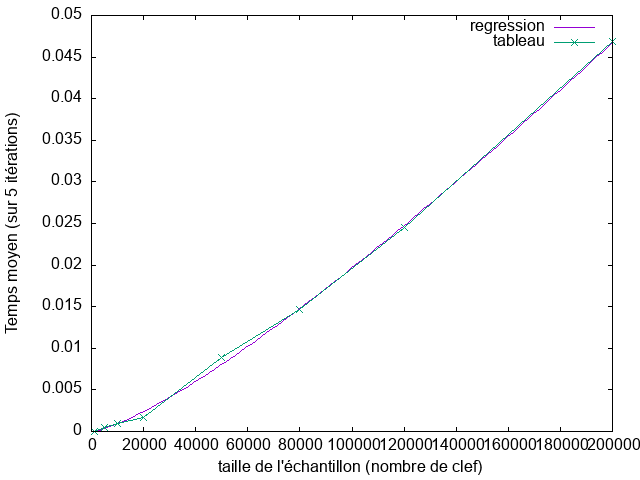
\includegraphics[scale=0.5]{../Images/svg courbes pour rapport/regression_ajout_iteratif_tab.png}
\caption{Mesure du temps pris par l'ajout itératif, tas sous forme de tableau}
\end{figure}

En observant la correspondance, il apparaît que l'ajout itératif sur le tableau semble être en $O(n log n)$.


\subsubsection{Tas implémenté avec une arborescence}

Nous obtenons la courbe et les paramètres pour la régression suivants : 


\begin{center}
\begin{tabular}{|c|c|c|c|c|}
\hline
 & a & b & c & m\\
\hline
coefficient & 1.37702e-08 & 
9.99416e-05 & 
-3862.02 & 
1.13792e+06 \\
Erreur asymptotique & +/- 5.828e-08 & +/- 0.0006326 & +/- 4.284e+10   & +/- 1.275e+08\\
\hline
\end{tabular}
\end{center}


\begin{figure}[hbtp]
\centering
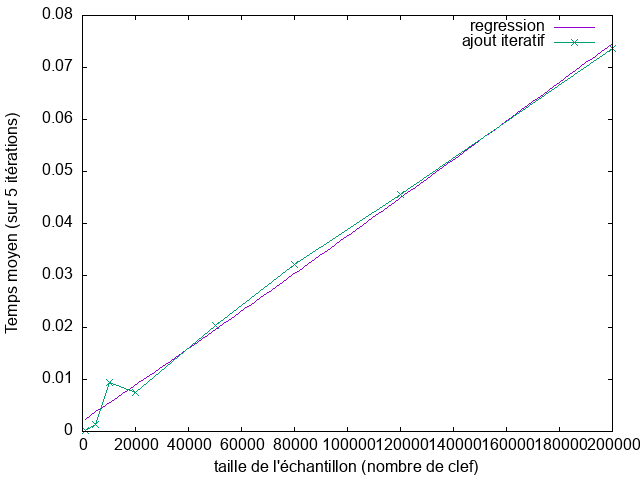
\includegraphics[scale=0.5]{../Images/svg courbes pour rapport/regression_ajout_iteratif_arbre.png}
\caption{Mesure du temps pris par l'ajout itératif, tas sous forme d'arbre}
\end{figure}

Notons ici que la régression linéaire est moins alignée avec nos différents points, mais la correspondance peut néanmoins nous faire considérer que l'ajout itératif implémenté par arborescence semble être en $O(n log n)$.




\subsection{\textit{construction}}

La complexité théorique de la fonction de construction, comme montré précédemment, est en $O(n)$, nous avons donc utilisé la fonction suivante pour l'ajuster à nos courbes avec les paramètres m et b : 

$$
f(x) = mx +b
$$

\subsubsection{Tas implémenté avec un tableau}

Nous obtenons la courbe et les paramètres pour la régression suivants : 

\begin{center}
\begin{tabular}{|c|c|c|}
\hline
 & m & b \\
\hline
coefficient & 3.38282e-07 & -0.00194051 \\
Erreur asymptotique & +/- 1.284e-08 & +/- 0.001147  \\
\hline
\end{tabular}
\end{center}


\begin{figure}[hbtp]
\centering
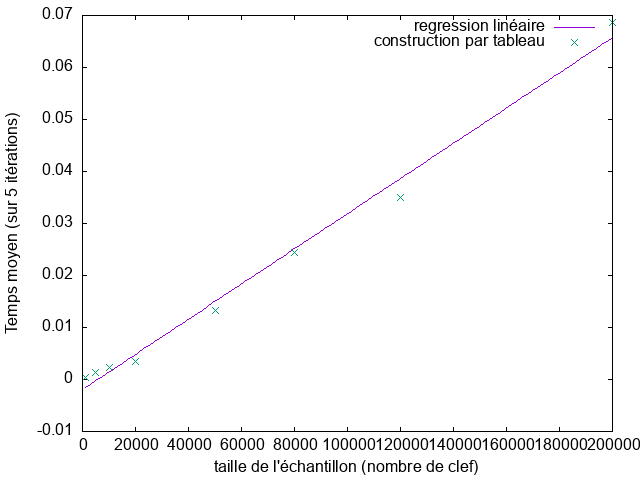
\includegraphics[scale=0.5]{../Images/svg courbes pour rapport/cplxt_cons_tab_regression.png}
\caption{Mesure du temps pris par la construction, tas sous forme de tableau}
\end{figure}

En observant la correspondance, il apparaît que la construction avec des tas implémentés par un tableau semble être en $O(n)$.


\subsubsection{Tas implémenté avec une arborescence}

Nous obtenons la courbe et les paramètres pour la régression suivants : 


\begin{center}
\begin{tabular}{|c|c|c|}
\hline
 & m & b \\
\hline
coefficient & 1.16615e-07 & 0.000263775 \\
Erreur asymptotique & +/- 3.17e-09 & +/- 0.0002832  \\
\hline
\end{tabular}
\end{center}


\begin{figure}[hbtp]
\centering
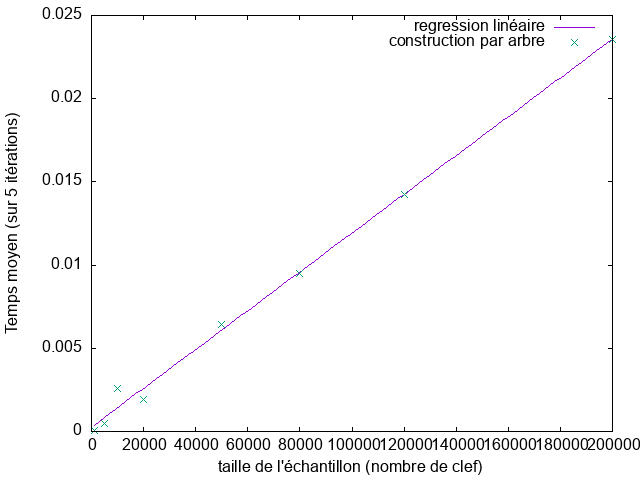
\includegraphics[scale=0.5]{../Images/svg courbes pour rapport/cplxt_cons_arbre_regression.png}
\caption{Mesure du temps pris par la construction, tas sous forme d'arbre}
\end{figure}

En observant la correspondance, il apparaît que la construction avec des tas implémentés par une arborescence semble être en $O(n)$.




\subsection{Vérification graphique pour l'union}

La complexité théorique de la fonction de l'union, comme montré précédemment, est en $O(n + m )$, nous avons donc utilisé la fonction suivante pour l'ajuster à nos courbes avec les paramètres m et b ( $x = n+m $): 

$$
f(x) = mx +b
$$

Pour nos jeux de tests, nous avons décidé de faire fixer à chaque fois l'union entre deux tas de même taille. Nous courbes représentent donc l'évolution du temps par l'algorithme pour fusionner deux tas de taille n, variant de 1000 à 2000000,  20 itérations servent à faire la moyenne (pour nos 5 jeux de données d'une taille précise, on fait la fusion avec les autres jeux de données uns par uns). Ce choix est dû au fait que pour estimer la complexité au pire cas de l'union, la seule donnée intéressante à faire varier est $n+m$, avec n la taille du premier tas et m celle du second, et pas la taille des deux tas prise individuellement\footnote{De premiers essais en fixant $n$ à 1000 nous ont montré une complexité similaire, il ne nous a pas semblé utile d'aller plus loin dans les expérimentations sur ce sujet}.

Notons également d'une rapide vérification avec la commande unix diff nous a permis de nous assurer que dans nos jeux de clés de même taille, il n'y avait aucune répétitions.


\subsubsection{Tas implémenté avec un tableau}

Nous obtenons la courbe et les paramètres pour la régression suivants : 


\begin{center}
\begin{tabular}{|c|c|c|}
\hline
 & m & b \\
\hline
coefficient & 3.86017e-07 & -0.00183903 \\
Erreur asymptotique & +/- 7.759e-09 & +/- 0.000693  \\
\hline
\end{tabular}
\end{center}


\begin{figure}[hbtp]
\centering
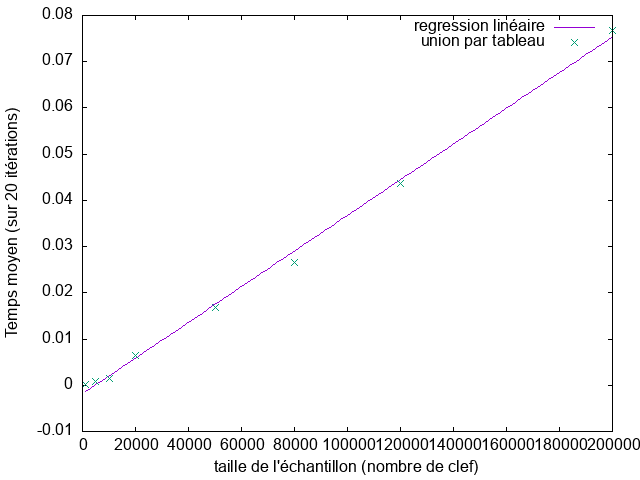
\includegraphics[scale=0.5]{../Images/svg courbes pour rapport/cplxt_union_tab_regression.png}
\caption{Mesure du temps pris par l'union, tas sous forme de tableau}
\end{figure}

En observant la correspondance, il apparaît que l'union avec des tas implémentés par un tableau semble être en $O(n)$.


\subsubsection{Tas implémenté avec une arborescence}

Nous obtenons la courbe et les paramètres pour la régression suivants : 


\begin{center}
\begin{tabular}{|c|c|c|}
\hline
 & m & b \\
\hline
coefficient & 3.97294e-07 &-0.00070037 \\
Erreur asymptotique & +/- 6.106e-09 & +/- 0.0005454  \\
\hline
\end{tabular}
\end{center}


\begin{figure}[hbtp]
\centering
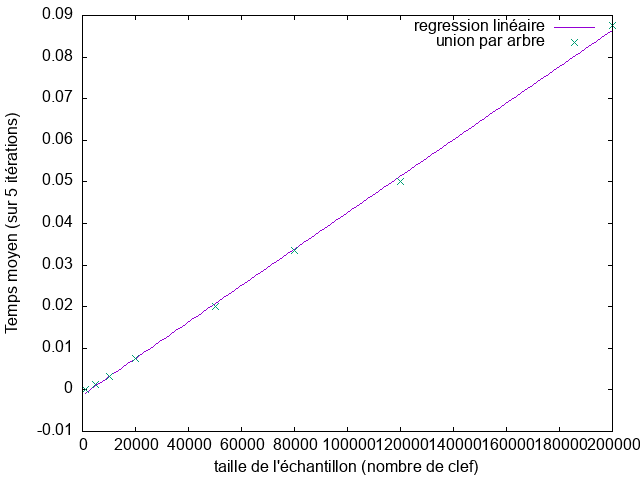
\includegraphics[scale=0.5]{../Images/svg courbes pour rapport/cplxt_union_arbre_regression.png}
\caption{Mesure du temps pris par l'union, tas sous forme d'arbre}
\end{figure}

En observant la correspondance, il apparaît que l'union avec des tas implémentés par une arborescence semble être en $O(n)$.


\subsection{Conclusion sur cette partie}

Ainsi, dans cette section, nous avons étudié deux manières d'implémenter un tas minimal : la manière usuelle et impérative, et une manière davantage compatible avec le style fonctionnel d'OCaml.

Il est alors intéressant de noter que le choix du langage a probablement pu influencer nos expérimentations, notamment sur les vitesses des opérations dans nos deux structures : le tas minimal sous forme d'arbre semble être plus rapide, en OCaml, du fait que le langage s'adapte très bien au style fonctionnel\footnote{notre hypothèse concernant cette notable différence est que le compilateur optimise plus facilement cette manière de faire que des parcours de tableau}.

Grâce à l'implémentation purement fonctionnelle sous forme d'arbre, nous avons pu nous confronter aux difficultés qu'il peut y avoir à manipuler ce type de structures dans ce paradigme de programmation, ce qui nous a fait essayer de comprendre plus en détail le fonctionnement d'un tas, et de chercher des propriétés dessus qui pourraient nous être utiles pour parcourir nos arbres de haut en bas par un chemin en $O(log n)$.

Nous avons également pu étudier une manière moins naïve de construire un tas minimal grâce à l'algorithme de Robert Floyd\cite{ACM}, ainsi qu'une approche plus poussée de la complexité au pire cas sur des tas minimum.

\section{File binomiale}

%TODO raconter la base des bases sur ce qu'est une file binomiale
Dans cette section, nous allons étudier l'implémentation en OCaml d'une file binomiale\cite{TasBinom}, et ce dans un style purement fonctionnel, ce qui s'accorde assez bien avec la structure.
Le code se trouve dans le fichier \textit{src/file\_binomiale}. 

\subsection{Primitives et structure}

Nous définissions sa structure, en OCaml, à l'aide de deux types récursifs : 

\begin{lstlisting}
(*Racine(degre,cle,fils)*)
type tournois_b = Racine of int * Int128.t * (tournois_b list)  | Empty 
(*File(indice,tournois) tournois le plus petit a droite de la liste *) 
type file_b = File of int * (tournois_b list) | Empty 
\end{lstlisting}

Nous définissons également les primitives suivante (leur code se trouve dans le fichier \textit{src/file\_binomiale.ml} :

\begin{lstlisting}
let est_vide_t (t : tournois_b) : bool = (*...*)

let degree (t:tournois_b) : int = (*...*)

let union2Tid (t1:tournois_b) (t2:tournois_b) : tournois_b = (*...*)

let rec  pow_2 (n:int) : int = (*...*)

let rec tournois_reverse (ol : tournois_b list ) (nl : tournois_b list): tournois_b list = (*...*)

let decapiter (t: tournois_b) : file_b = (*...*)

let file(t:tournois_b) : file_b = (*...*)

let est_vide_f (f: file_b ) : bool = (*...*)

let rec last_tournois  (li : tournois_b list) : tournois_b = (*...*)

let mindeg (f:file_b) : tournois_b = (*...*)

let reste (f:file_b) : file_b = (*...*)

let ajout_min (t:tournois_b) (f:file_b) : file_b = (*...*)
\end{lstlisting}

\subsection{Fonctions fondamentales}

\subsection{Vérification graphique de la complexité de construction}

\subsection{Vérification graphique de la complexité de union}


\section{Hachage}

\section{Arbre Binaire de Recherche}

\section{Étude expérimentale}



\cleardoublepage

\addcontentsline{toc}{section}{Bibliographie}
\bibliography{biblio.bib}
\bibliographystyle{plain}
\nocite{*}


\end{document}